\documentclass{standalone}
%% Show/hide steps for standalone work — edit this line:
\makeatletter\AtBeginDocument{\@buildstepset{1,2,3,4,5}}\makeatother
\usepackage{tikz}
\usepackage{hsbcommon}
\begin{document}
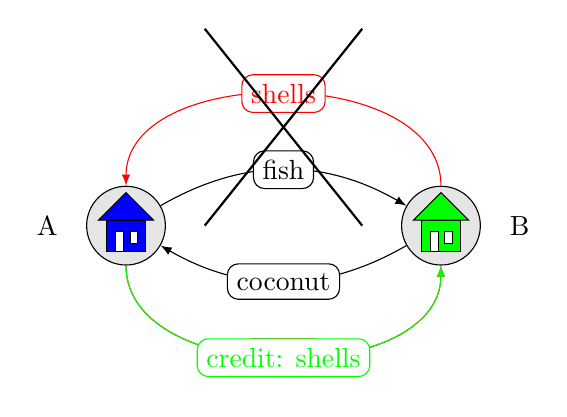
\begin{tikzpicture}
        \tikzset{
            myhome/.pic={
            \begin{scope}[xshift=-0.25cm,yshift=-0.33cm]
                    
                \filldraw (-0,0) rectangle (0.5,0.4);
                \filldraw (-0.1,0.4) -- (0.25,0.75) -- (0.6,0.4) -- cycle;
                \filldraw[white,draw=black] (0.12,0) rectangle (0.22,0.25);
                \filldraw[white,draw=black] (0.3,0.1) rectangle (0.4,0.25);
            \end{scope}
            }
        }
        \coordinate (A) at (-2,0);
        \coordinate (B) at ( 2,0);
        \node[draw, fill=gray!20, circle, minimum width=1cm] (NA) at (A) {}; \node[left of=A] {A};
        \node[draw, fill=gray!20, circle, minimum width=1cm] (NB) at (B) {}; \node[right of=B] {B};
        \draw[fill=blue] (A) pic {myhome};
        \draw[fill=green] (B) pic {myhome};

        %%% make sure canvas size is always the same

        \phantom{
            \draw[->,>=latex] (NA) [out=90,in=90] to node[draw,rounded corners, fill=white] {shells} (NB);
        }
        
        %%% FISH
        \ifstep{1}{
            \draw[->,>=latex] (NA) [out=30,in=150] to node[draw,rounded corners, fill=white] {fish} (NB);
        }       
        %%% COCONUT
        \ifstep{2}{
            \draw[<-,>=latex] (NA) [out=-30,in=-150] to node[draw,rounded corners, fill=white] {coconut} (NB);
        }
     
        %%% SHELLS FOR FISH
        \ifstep{3}{
        \begin{scope}[color=red]
            \draw[<-,>=latex] (NA) [out=90,in=90] to node[draw,rounded corners, fill=white] {shells} (NB);
        \end{scope}
        }

        %%% SHELLS FOR COCONUT
        \ifstep{4}{
        \begin{scope}[color=red]
            \draw[->,>=latex] (NA) [out=-90,in=-90] to node[draw,rounded corners, fill=white] {shells} (NB);
        \end{scope}
        }

        %%% Crossing out fish against shells
        \ifsteponly{1,3}{2,4,5}{
            \draw[thick] (-1,2.5) -- (1,0);
            \draw[thick] (-1,0) -- (1,2.5);
        }

        %%% Debt instead of shells
        \ifsteponly{5}{4}{
            \begin{scope}[color=green]
                \draw[->,>=latex] (NA) [out=-90,in=-90] to node[draw,rounded corners, fill=white] {credit: shells} (NB);
            \end{scope}
        }
        
        
\end{tikzpicture}
\end{document}
